% Copyright 2022 by Marek Rychly <rychly@fit.vut.cz>.
%
\documentclass[10pt,xcolor=pdflatex,dvipsnames,table,oneside]{book}
% babel and encoding
\usepackage[slovak]{babel}
\usepackage[T1]{fontenc}
\usepackage[utf8]{inputenc}

\usepackage{csquotes}% correct/formal language-specific quotations
\usepackage{microtype}% character protrusion, font expansion, adjustment of interword spacing, additional kerning, tracking, etc.
\usepackage{hyperref}% hyper-refs in PDF
\usepackage{graphicx}
\usepackage{caption}
\usepackage{placeins}

\author{
  Marek Mudroň\\
  \texttt{xmudro04}
  \and
  Samuel Repka\\
  \texttt{xrepka07}
  \and
  Barbora Šmahlíková\\
  \texttt{xsmahl00}
}
\title{Príprava dát a ich popisná charakteristika}
\date{zima 2022}

\begin{document}

\pagenumbering{roman}

\hypersetup{pageanchor=false}% disable hyperref anchor to title page as maketitle enforce pagenumbering to arabic which colides the titlepage with the first arabic page below
\maketitle
\hypersetup{pageanchor=true}
\tableofcontents

\newpage% force page-break to start the page numbering on a new page
\pagenumbering{arabic}


\chapter{Dátová sada}

V tomto projekte sa zaoberáme exploráciou, čistením a tvorbou popisnej charakteristiky pre open-source dátovú sadu
\textit{Palmer Archipelago (Antarctica) penguin data}. Ide o dátovú sadu, ktorej obsahom sú informácie o fyziologických a demografických vlastnostiach troch druhov tučniakov. Dataset obsahuje súbory \texttt{penguins\_lter.csv} a \texttt{penguins\_size.csv}. Oba obsahujú informácie k rovnakým jedincom,  no \texttt{penguins\_lter.csv} poskytuje okrem informácií obsiahnutých v \texttt{penguins\_size.csv} aj dáta k hodnotám stabilných izotopov uhlíka  ($\delta^{13}$C)  a dusíka  ($\delta^{15}$N)  v tele. Tieto údaje sa používajú už od roku 1980  poskytujú hodnotné informácie k životospráve a migračným vzorcom tučniakov. Preto pre naše účely využívame informácie obsiahnuté v \texttt{penguins\_lter.csv}.

\chapter{Exploratívna analýza}
Táto kapitola sa venuje
\section{Atribúty}

\subsection*{studyName}
Tento atribút obsahuje identifikátor štúdie, z ktorej dáta pochádzajú. Celkovo sú identifikátory tri, a to \texttt{PAL0708}(s počtom 110), \texttt{PAL0809}(114 prvkov) a \texttt{PAL0910}(počet prvkov 120).

\subsection*{Sample Number}
Poradové číslo záznamu vzťahujúce sa na konkrétnu štúdiu.

\subsection*{Species}
Dataset obsahuje v atribúte \texttt{Species} názov jedného z troch druhov tučniakov
\begin{itemize}
  \item Adelie Penguin (Pygoscelis adeliae)
  \item Chinstrap penguin (Pygoscelis antarctica)
  \item Gentoo penguin (Pygoscelis papua)
\end{itemize}


V dátach dominuje Adelie penguin, nasledovaný tučniakom Gentoo a Chinstrap, ako je vidieť na grafe \ref{fig:species_graph}.
\begin{figure}[h]
  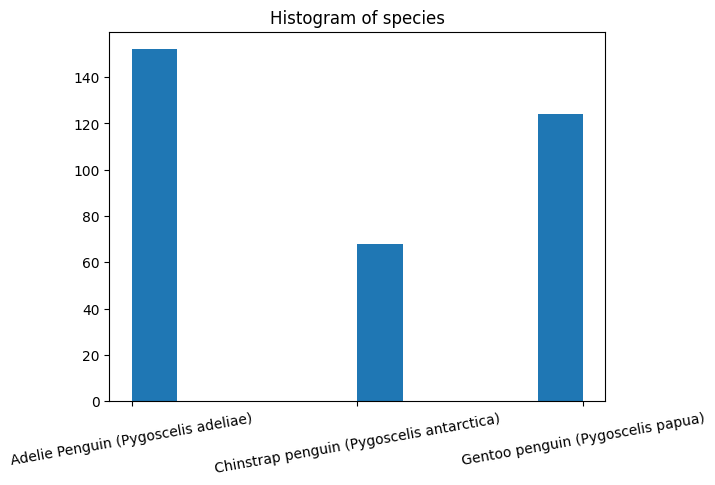
\includegraphics[width=9cm]{img/species.png}
  \centering
  \caption{Histogram počtu tučniakov podľa druhu}
  \label{fig:species_graph}
\end{figure}


\subsection*{Region}
V atribúte \texttt{Region} je uvedená oblasť výskytu daného jedinca. Táto je pre každého z nich rovnaká a obsahuje hodnotu \textit{Anvers}.


\subsection*{Island}
Informácia obsiahnutá v tomto atribúte označuje ostrov, ktorý obýva jedinec na zázname. Demografické rozloženie sa medzi druhmi líši, ako je vidno na grafe \ref{fig:counts}.
Atribút obsahuje tieto tri hodnoty.
\begin{itemize}
  \item Torgersen
  \item Biscoe
  \item Dream
\end{itemize}

\begin{figure}[h]
  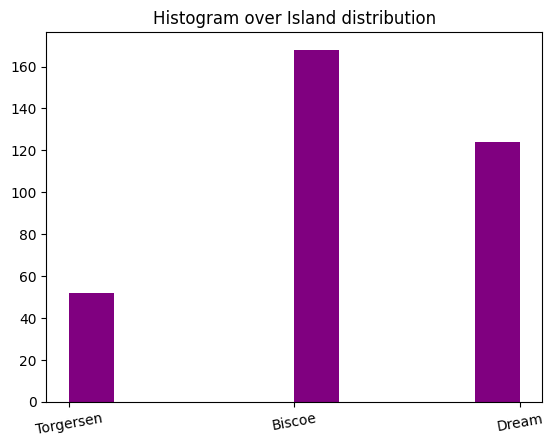
\includegraphics[width=7.5cm]{img/island.png}
  \centering
  \caption{Počty tučniakov na ostrovoch, ako sú uvedené v datasete.}
  \label{fig:counts}
\end{figure}



\subsection*{Stage}
Atribútom \texttt{Stage} uvádza pre každého jedinca rovnakú hodnotu \textit{Adult,~1~Egg~Stage}.


\subsection*{Individual ID}
Identifikátor každého z jedincov. Neexistuje záznam bez tejto hodnoty. V datasete sa ale nachádza len 190 unikátnych identifikátorov, pričom celkový počet záznamov je 344.


\subsection*{Clutch completion}
\texttt{Clutch Completion} obsahuje informáciu o tom, či bol jedince pozorovaný s hniezdom obsahujúcim 2 vajíčka. Obsahuje
hodnoty, "Yes" a "No". Skoro 90\% jedincov má v záznamoch uvedené "Yes".


\subsection*{Date egg}
Dátum, kedy bolo hniezdo prvý krát pozorované s 1 vajíčkom.


\subsection*{Culmen length (mm) a Culmen depth (mm)}
Atribúty \texttt{Culmen Length (mm)} a  \texttt{Culmen Depth (mm)} poskytujú rozmery zobáku. Culmen length označuje jeho dĺžku v milimetroch, zatiaľ čo Culmen depth označuje jeho výšku. Hodnoty pre Culmen length sú v intervale od 32.1 do 59.6 mm, so strednou hodnotou 43.92mm a štandardnou odchýlkou 5.46. Culmen depth má hodnoty od 13.1 do 21.5 mm, stredná hodnota 17.15 a odchýlka 1.97.


\subsection*{Flipper length (mm)}
Dĺžka krídel tučniaka je obsiahnutá v atribúte \texttt{Flipper Length (mm)} a taktiež je v milimetroch. Stredná hodnota je 200.9 mm, so štandardnou odchýlkou 14 mm. Namerané maximum je 231 mm a minimum 172 mm.


\subsection*{Body mass (g)}
Telesnú hmotnosť v gramoch poskytuje atribút \texttt{Body Mass (g)}. Najtučnejší tučniak váži 6.3 kg. Na druhom konci spektra sa nachádza tučniak s hmotnosťou 2.7 kg. Stredná hodnota je 4.2 kg a štandardná odchýlka 0.8 kg.


\subsection*{Sex}
Pohlavie jedinca. Táto hodnota nie je vždy uvedená, a v jednom prípade jedna z položiek tohto atribútu obsahuje nevalidnú hodnotu '.' \ref{fig:the_thing}.

\begin{figure}[t]
  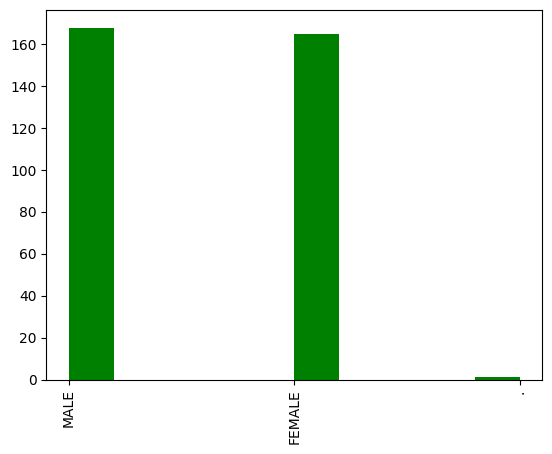
\includegraphics[width=8cm]{img/the_thing.png}
  \centering
  \caption{Histogram pohlaví tučniakov s nevyfiltrovanou nevalidnou hodnotou.}
  \label{fig:the_thing}
\end{figure}


\subsection*{Delta 15 N (o/oo)}
Stabilný izotop dusíka. Meranie tohoto atribútu prebehlo 330 krát. Stredná hodnota je 8.73 so štandardnou odchýlkou 0.551. Namerané maximum je 10.03 a minimum 7.63.


\subsection*{Delta 13 C (o/oo)}
Atribút s meraniami stabilných izotopov uhlíka. Podobne ako pri Delta 15 N, dataset obsahuje 330 záznamov s týmito hodnotami. Stredná hodnota je -25.69 a štandardná odchýlka 0.79. Maximum je -23.787 a minimum je -27.02.


\subsection*{Comments}
Tento atribút je pomerne zriedka vyplnený a obsahuje slovné poznámky k niektorým meraniam. Z hľadiska strojového spracovania dát je irelevantný.

\newpage
\section{Analýza vzťahov}
Na získanie prvotného pohľadu na vzťahy sme vytvorili korelačnú maticu \ref{fig:corr}. Môžeme z nej vyčítať rôzne informácie, ako napríklad že hmotnosť je silno korelovaná s dĺžkou krídel, čo sa dá intuitívne čakať. Nie až také intuitívne je, že výška zobáka je trochu inverzne korelovaná s dĺžkou krídel.

\begin{figure}[h]
  \centering
  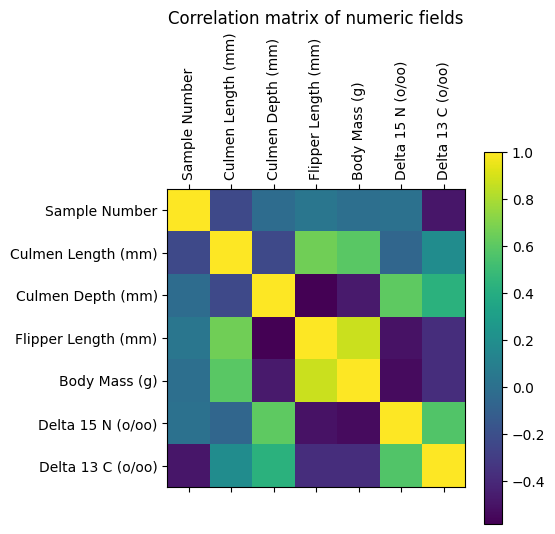
\includegraphics[width=8cm]{img/corr.png}
  \caption{Korelačná matica číselných atribútov}
  \label{fig:corr}
\end{figure}
\FloatBarrier

Bližší náhľad na koreláciu hmotnosti a dĺžky krídlel nám poskytol graf \ref{fig:flbm}. Vidno, že na atribútoch existuje pomerne silná závislosť, ktorá sa dá aproximovať priamkov (aj keď nie veľmi presne.)
\begin{figure}[h]
  \centering
  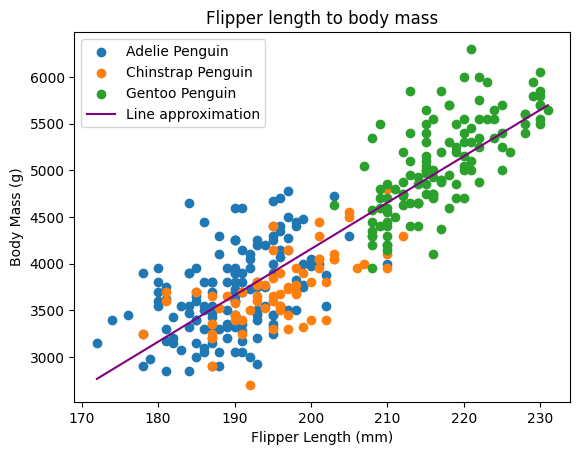
\includegraphics[width=8cm]{img/flbm.png}
  \caption{Dĺžka krídel vzhľadom k hmotnosti}
  \label{fig:flbm}
\end{figure}
\FloatBarrier

Zaujímavý je aj pohľad na dáta z hľadiska druhov, teda ktorý druh obýva ktorý ostrov. Bol predpoklad, že jeden druh obýva len jeden ostrov. Graf \ref{fig:islanddist} to do istej miery aj potvrdzuje, pretože tučniaky druhu Chinstrap a Gentoo sa naozaj nachádzajú len na jednom ostrove. Druh Adelie je ale na všetkých.
\begin{figure}[h]
  \centering
  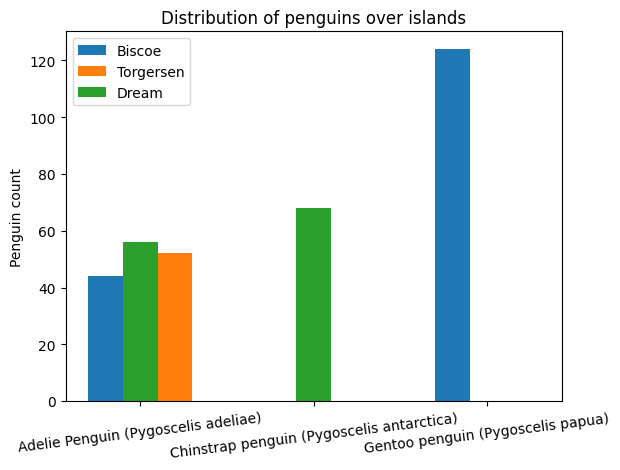
\includegraphics[width=8cm]{img/distribution_species.png}
  \caption{Distribúcia druhov po ostrovoch}
  \label{fig:islanddist}
\end{figure}

Vzťah medzi dĺžkou a výškou zobáka je niečo, čo by človek prirodzene čakal. Napriek tomu korelácia je takmer nulová.  Po vygrafovaní týchto parametrov vznikol pomerne chaotický graf, ktorý ale okamžite začal dávať zmysel pri dodatočnom rozdelení podľa druhu (Fig \ref{fig:clusters}). Na obrázku je jasne vidieť zhluky bodov, zodpovedajúce jednotlivým druhom. Rozmery zobáka by mohli byť potenciálne klasifikačné kritérium druhu.
\begin{figure}[h]
  \centering
  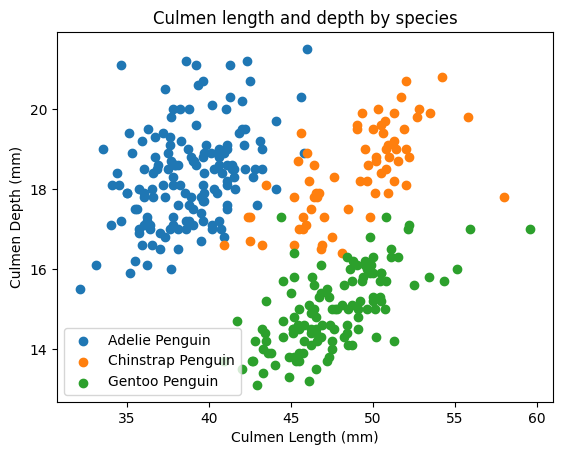
\includegraphics[width=7.6cm]{img/clcd.png}
  \caption{Porovnanie výšky a dĺžky zobáka vzhľadom ku druhu.}
  \label{fig:clusters}
\end{figure}
\FloatBarrier

Pre porovnanie distribúcií hmotností podľa druhu sa hodí husľový graf, ako vidno na \ref{fig:violin}. Prekvapivo to vyzerá, že jednotlivé druhy majú pomerne odlišné distribúcie.
\begin{figure}[h]
  \centering
  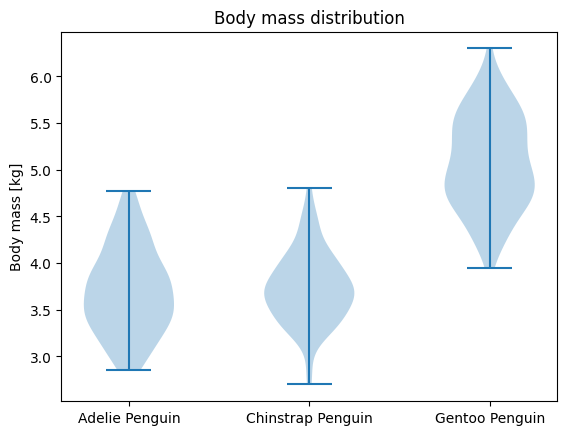
\includegraphics[width=7.8cm]{img/bmdist.png}
  \caption{Husľový graf znázorňujúci distribúcie hmotností tučniakov rozdelených podľa druhu.}
  \label{fig:violin}
\end{figure}

Posledný vzťah, na ktorý sme sa pozreli ako potenciálneho kandidáta na klasifikáciu druhu, bol čas kladenia vajec. Na tento účel sme spravili histogram \ref{fig:egg}, na ktorom ale vidno, že všeky druhy kladú vajcia v priibližne rovnakom čase.
\begin{figure}[h]
  \centering
  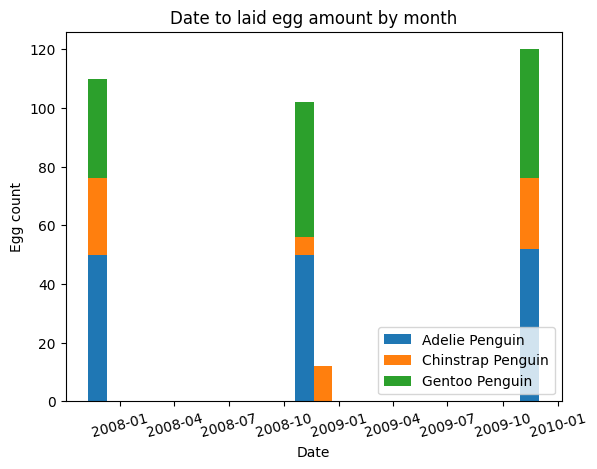
\includegraphics[width=8cm]{img/date_egg.png}
  \caption{Histogram kladenia vajec vzhľadom na čas}
  \label{fig:egg}
\end{figure}


\FloatBarrier
\section{Odlehlé hodnoty}
Odlehlé hodnoty v datové sadě jsme hledali pomocí mezikvartilového rozpětí (IQR). Pro odlehlou hodnotu musí platit, že je menší než $q_1 - 1.5 \cdot \textrm{IQR}$ nebo větší než $q_3 + 1.5 \cdot \textrm{IQR}$, kde $q_1$ a $q_3$ jsou hodnoty prvního a třetího kvartilu. Takové hodnoty má smysl hledat pouze u numerických atributů.

Pro žádný z atributů jsme nenašli odlehlé hodnoty, když jsme uvažovali celou datovou sadu. Jelikož se ale hodnoty atributů jako délka křídel a zobáku určitě liší v závislosti na druhu tučňáka, rozhodli jsme se hledat odlehlé hodnoty atributů pro jednotlivé druhy tučňáků.
Tam už jsme odlehlé hodnoty našli.


\section{Chybějící hodnoty}
\begin{table}[]
  \centering
  \begin{tabular}{|l|l|l|l|l|l|l|l|l|}
    \hline
    \textbf{Název atributu} & \textbf{Počet chybějících hodnot} \\ \hline
    Name                    & 0 / 344                           \\ \hline
    Sample number           & 0 / 344                           \\ \hline
    Species                 & 0 / 344                           \\ \hline
    Island                  & 0 / 344                           \\ \hline
    Stage                   & 0 / 344                           \\ \hline
    Individual ID           & 0 / 344                           \\ \hline
    Clutch completion       & 0 / 344                           \\ \hline
    Date egg                & 0 / 344                           \\ \hline
    Sex                     & 10 / 344                          \\ \hline
    Comments                & 318 / 344                         \\ \hline
    Culmen length           & 2 / 344                           \\ \hline
    Culmen depth            & 2 / 344                           \\ \hline
    Flipper length          & 2 / 344                           \\ \hline
    Body mass               & 2 / 344                           \\ \hline
    Delta 13                & 13 / 344                          \\ \hline
    Delta 15                & 14 / 344                          \\ \hline
  \end{tabular}
  \caption{Počty chybějících hodnot}
  \label{tab:missing}
\end{table}

Dále jsme zkoumali počet chybějících hodnot u jednotlivých atributů. Výsledky analýzy jsou uvedeny v tabulce \ref{tab:missing}.
Celkově chybí 35 numerických hodnot, 10 hodnot u pohlaví tučňáka a 318 komentářů. Chybějící komentáře ovšem nejsou důležité, obsahují pouze nějakou přidanou informaci a neočekává se, že by tato hodnota měla být přítomna u všech tučňáků.

Pokud pomineme atribut \texttt{Comments}, je zcela vyplněných řádků v tabulce 325, těch kde tedy chybí alespoň jedna hodnota je 19. (Řádků, které jsou zaplněny zcela, včetně komentářů, je 13.)
Z celkových 19 řádků je 13 řádků, ve kterých chybí hodnota více než jednoho atributu. Nejvíce hodnot chybí na řádku 3 a 339 (což odpovídá řádkům 5 a 341 po otevření v Excelu) -- na každém z těchto řádků je 7 chybějících hodnot.



\chapter{Príprava dátovej sady pre dolovacie algoritmy}
% Barbora s tymto ti nepomozem :)


\end{document}
